\documentclass[conference]{IEEEtran}

\IEEEoverridecommandlockouts

\usepackage{cite}
\usepackage{graphicx}
\usepackage{amsmath,amssymb}
\usepackage{url}
\usepackage{booktabs}

\title{Autonomous Plant Irrigation System Using ESP32 and Soil Moisture Sensing}

\author{\IEEEauthorblockN{Niroop Baliji}
\IEEEauthorblockA{Department of Automobile Engineering\\
VNR VJIET\\
Hyderabad, India\\
Email: your.email@example.com}}

\begin{document}

\maketitle

\begin{abstract}
Small-scale plant care often depends on manual irrigation, which introduces inconsistent watering frequency and avoidable water wastage. This paper presents an ESP32-based autonomous irrigation controller that combines soil moisture sensing, ambient monitoring, and tank-level safety checks to make local watering decisions without cloud dependency. The implementation follows a dual-track workflow: modular firmware for physical deployment and a Wokwi digital twin for repeatable simulation and fast validation. The control logic activates pumping only when soil moisture is below threshold and tank-water availability is confirmed. To improve operational safety, tank interlock, cooldown delay, and watchdog timeout mechanisms are integrated. Validation in the digital twin demonstrates expected behavior for wet-soil hold, dry-soil activation, and tank-empty safety override. The approach emphasizes reliability, reproducibility, and low-cost implementation suitable for student projects and early prototype deployment.
\end{abstract}

\begin{IEEEkeywords}
ESP32, IoT, smart irrigation, embedded control, safety interlock
\end{IEEEkeywords}

\section{Introduction}
Irrigation automation is a practical embedded-systems application for low-cost agriculture and home gardening. Manual watering is often inconsistent and can result in under-watering, over-watering, and poor resource utilization. This work targets a compact ESP32-based architecture that performs local autonomous decisions using sensor data and deterministic control logic.

The proposed controller uses soil moisture as the primary irrigation trigger, while DHT22 temperature and humidity readings provide environmental context. A tank-level input prevents pump dry-run by blocking irrigation when water is unavailable. The project contribution is a dual-track engineering approach: deployment-oriented modular firmware and a simulation twin for repeatable verification.

\section{Literature Survey}
Typical IoT irrigation literature focuses on three axes: sensing reliability, control strategy, and communication design. Many low-cost systems employ threshold control because of implementation simplicity, while advanced systems incorporate weather prediction or ML-based optimization. Safety handling is frequently limited in small prototypes, especially for dry-run prevention and fail-safe actuation behavior.

Compared to cloud-first solutions, local-decision systems are easier to reproduce in constrained academic environments and remain functional during connectivity interruptions. This project prioritizes control correctness and safety sequencing first, with cloud telemetry treated as future work.

\section{System Architecture}
The architecture is split into three layers:
\begin{enumerate}
    \item Embedded firmware layer for physical deployment.
    \item Wokwi digital twin layer for deterministic validation.
    \item Documentation layer for traceable evidence and reporting.
\end{enumerate}

The hardware stack includes ESP32 DevKit V1, a capacitive soil sensor, DHT22, relay-based pump control, and a tank-level switch. Firmware modules separate configuration, sensing, irrigation decisions, and telemetry outputs.

\begin{figure}[!t]
\centering
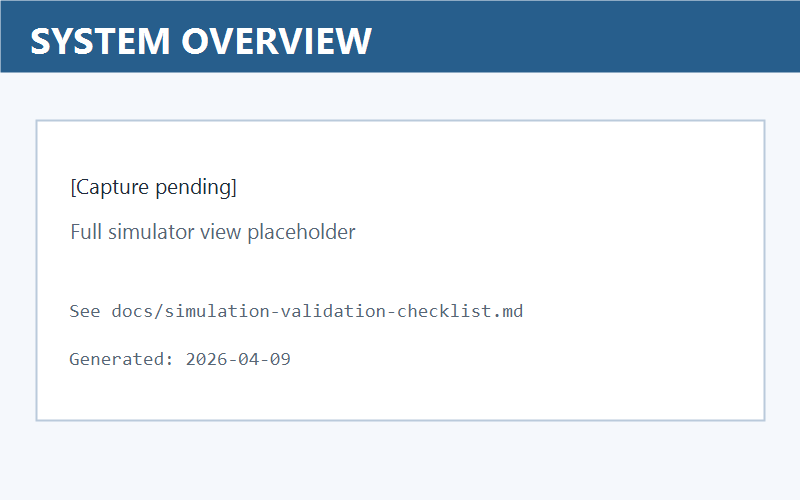
\includegraphics[width=0.95\linewidth]{../../docs/images/system-overview.png}
\caption{Digital twin system overview (placeholder to be replaced with final validation capture).}
\label{fig:system_overview}
\end{figure}

\section{Implementation}
\subsection{Hardware Design}
The implementation uses GPIO34 for soil moisture analog input, GPIO4 for DHT22 data, GPIO5 for tank-level input, and GPIO18 for relay output. In production configuration, relay polarity is active-high, while the Wokwi relay model is active-low. This difference is documented in simulation code comments to avoid deployment mistakes.

\subsection{Firmware Design}
The control loop performs periodic sensing and state updates. Key tunable parameters include soil dryness threshold, pump ON duration, cooldown period, and watchdog timeout. Controller states include monitoring, watering, cooldown, and error handling. Telemetry logs timestamped values and decision outputs for traceability.

\subsection{Safety Mechanisms}
The controller enforces three safeguards:
\begin{enumerate}
    \item Tank interlock to block pumping if water is unavailable.
    \item Cooldown delay to avoid frequent relay toggling.
    \item Watchdog timeout to force pump shutdown on abnormal runtime.
\end{enumerate}

\section{Simulation and Testing}
Validation is executed through a checklist-driven Wokwi process. Core scenarios include wet-soil baseline hold, dry-soil pump activation, and tank-low interlock behavior. Serial telemetry is used as decision evidence and paired with screenshot captures.

\begin{table}[!t]
\caption{Validation Scenario Outcomes (Fill with Final Measurements)}
\label{tab:validation}
\centering
\begin{tabular}{@{}llll@{}}
\toprule
Scenario & Expected & Observed & Pass/Fail \\
\midrule
Wet soil baseline & pump OFF & [fill] & [fill] \\
Dry soil & pump ON & [fill] & [fill] \\
Tank low interlock & pump OFF & [fill] & [fill] \\
Cooldown behavior & sequence seen & [fill] & [fill] \\
\bottomrule
\end{tabular}
\end{table}

\section{Results and Discussion}
Preliminary digital twin testing confirms expected state transitions for the primary scenarios. The pump remains off for wet conditions, activates when soil is dry, and is correctly blocked when tank level is low. Cooldown and watchdog logic improve operational safety over basic threshold-only actuation.

Current limitations include pending long-duration hardware measurements and placeholder evidence that must be replaced with final captures. The final manuscript should include quantitative values for activation success rate, interlock success rate, and timing consistency.

\section{Conclusion and Future Work}
This work demonstrates a reproducible, low-cost ESP32 irrigation controller with explicit safety mechanisms and simulation-backed validation. The architecture supports incremental development from digital twin verification to physical prototype deployment.

Future work includes hardware calibration, multi-day field evaluation, and optional cloud telemetry integration for long-term analysis.

\section*{Acknowledgment}
The author acknowledges guidance and support from the department and peers during iterative design and validation.

\bibliographystyle{IEEEtran}
\bibliography{references}

\end{document}
